%\documentclass{cumcmthesis}
\documentclass[withoutpreface,bwprint]{cumcmthesis} %去掉封面与编号页,电子版提交的时候使用。


\usepackage[framemethod=TikZ]{mdframed}
\usepackage{url}   % 网页链接
\usepackage{subcaption} % 子标题
\usepackage{amsmath}
\iffalse\usepackage{graphicx} %插入图片的宏包
\usepackage{float} %设置图片浮动位置的宏包
\usepackage{subfigure} %插入多图时用子图显示的宏包

\title{全国大学生数学建模竞赛编写的 \LaTeX{} 模板}
\tihao{A}
\baominghao{4321}
\schoolname{XX大学}
\membera{ }
\memberb{ }
\memberc{ }
\supervisor{ }%辅导老师
\yearinput{2023}
\monthinput{9}
\dayinput{8}

\begin{document}

 \maketitle
 \begin{abstract}
cumcmthesis 是为全国大学生数学建模竞赛编写的\LaTeX{}模板, 旨在让大家专注于 论文的内容写作, 而不用花费过多精力在格式的定制和调整上. 本手册是相应的参考, 其 中提供了一些环境和命令可以让模板的使用更为方便. 同时需要注意, 使用者需要有一 定的 \LaTeX{} 的使用经验, 至少要会使用常用宏包的一些功能, 比如参考文献,数学公式,图片使用,列表环境等等. 例子文件参看 \texttt{example.tex}.

\begin{mdframed} [%
	roundcorner=5pt,
	linecolor=gray!50,
	outerlinewidth=0.5pt,
	middlelinewidth=0.3pt, backgroundcolor=gray!2,
innertopmargin=\topskip, frametitle={2023 年建模比赛格式变化说明},
frametitlefont= \bfseries,frametitlerule=true,frametitlealignment =\raggedright\noindent,
frametitlerulewidth=.5pt, frametitlebackgroundcolor=gray!2,]
今年的格式变化主要就是一个地方,如下:
\begin{enumerate}
\item 论文第一页为承诺书,\textbf{\color{red}内容进行了调整}。

 

\end{enumerate}

\end{mdframed}


\url{https://www.latexstudio.net} 陆续推出了更优质的资源,欢迎学习 。

欢迎大家到QQ群里沟通交流:91940767/478023327/640633524。我们也开通了问答区交流 \LaTeX{}技术:\url{https://ask.latexstudio.net},欢迎大家前来交流,有问题就来这里,与大神零距离。

\uwave{关注我们的微信公众号}:

\centerline{
\includegraphics[width=6cm]{gongzhonghao2}}

\keywords{\TeX{}\quad  图片\quad   表格\quad  公式}
\end{abstract}

%目录  2019 明确不要目录,我觉得这个规定太好了
%\tableofcontents

%\newpage

\section{模板的基本使用}

要使用 \LaTeX{} 来完成建模论文,首先要确保正确安装一个 \LaTeX{} 的发行版本。

\begin{itemize}
    \item Mac 下可以使用 Mac\TeX{}
    \item Linux 下可以使用 \TeX{}Live ;
    \item windows 下可以使用 \TeX{}Live 或者 Mik\TeX{} ;
\end{itemize}

具体安装可以参考 \href{https://github.com/OsbertWang/install-latex-guide-zh-cn/releases/}{Install-LaTeX-Guide-zh-cn} 或者其它靠谱的文章。另外可以安装一个易用的编辑器,例如 \href{https://mirrors.tuna.tsinghua.edu.cn/github-release/texstudio-org/texstudio/LatestRelease/}{\TeX{}studio} 。

使用该模板前,请阅读模板的使用说明文档。下面给出模板使用的大概样式。

%\begin{tcode}
 \fi
   % \documentclass{cumcmthesis}
    %\documentclass[withoutpreface,bwprint]{cumcmthesis} %去掉封面与编号页

    \title{论文题目}
    \tihao{A}            % 题号
    \baominghao{4321}    % 报名号
    \schoolname{你的大学}
    \membera{成员A}
    \memberb{成员B}
    \memberc{成员C}
    \supervisor{指导老师}
    \yearinput{2017}     % 年
    \monthinput{08}      % 月
    \dayinput{22}        % 日

    \begin{document}
        \maketitle
        \begin{abstract}
            摘要的具体内容。
            \keywords{关键词1\quad  关键词2\quad   关键词3}
        \end{abstract}
        %\tableofcontents
        \section{问题重述}
        \subsection{问题背景}
        在移动互联网高速发展的背景下,“拍照赚钱”作为一种创新的自助式服务模式应运而生。其运作逻辑清晰且便捷:用户通过下载特定APP并完成注册成为会员后,可从平台领取各类需实地拍摄的任务——例如前往超市核查某款商品的上架状态,完成任务并通过审核后,即可获得平台预先标定的酬金。这类依托移动互联网搭建的自助式劳务众包平台,为企业提供了高效的商业检查与信息搜集解决方案。相较于传统市场调查模式,它凭借分散化的用户力量,大幅降低了企业的调查成本;同时,基于真实场景的实地拍摄机制有效保障了数据的真实性,且任务分发与回收的即时性显著缩短了调查周期,因此在商业领域得到广泛应用。  在此模式中,如何制定合理的任务定价,以平衡企业成本与用户参与度,确保任务能够高效完成,是需要解决的关键问题。
        \subsection{问题的提出}
        为研究合理的任务定价,提出了以下问题:
        \begin{enumerate}[
        label = (\arabic*),
        itemindent = 0pt,
        labelindent = \parindent,
        labelwidth = 2em,
        labelsep = 5pt,
        leftmargin = *]
        \item 研究附件一中项目的任务定价规律,分析任务未完成的原因。
        \item 为附件一中的项目设计新的任务定价方案,并和原方案进行比较。
        \item 实际情况下,多个任务可能因为位置比较集中,导致用户会争相选择,一种考虑是将这些任务联合在一起打包发布。在这种考虑下,如何修改前面的定价模型,对最终的任务完成情况又有什么影响?
        \item 对附件三中的新项目给出你的任务定价方案,并评价该方案的实施效果。
        \end{enumerate}
        \section{模型的假设}
        \begin{enumerate}[
        label = (\arabic*),
        itemindent = 0pt,
        labelindent = \parindent,
        labelwidth = 2em,
        labelsep = 5pt,
        leftmargin = *] 
        \item 假设任意两点间的实际路程可以用两点间的直线距离代替。
        \item 假设会员在接取任务后一定会将其完成,即任务完成率仅由接取率决定,排除用户接取后因主观放弃或客观障碍导致的未完成情况,简化完成率的计算逻辑。
        \item 假设任务的有效期足够长,且发布时间对用户接取意愿的影响可忽略不计,即假设所有任务在同一时间窗口内可供用户选择,排除时间因素对定价与完成率的干扰。
        \end{enumerate}
        \section{符号说明}
        \begin{center}
            \begin{tabular}{cc}
                \hline
                \makebox[0.3\textwidth][c]{符号}	&  \makebox[0.4\textwidth][c]{意义} \\ \hline
                $H_i$	    & 任务$i$的难易程度 \\ 
                $h_i$	    & 任务$i$经过离散化的难易程度 \\ 
                $MD_i$	    & 任务$i$周围的成员密度 \\ 
                $TD_i$	    & 任务$i$周围的任务密度 \\
                $S_{ij}$	    & 成员$j$对任务$i$的满意度 \\ 
                $P_{ij}$	    & 成员$j$对任务$i$的接取概率 \\ 
                $E_i$	    & 任务$i$所在城市成员对该任务的喜好程度 \\ 
                $q_i$	    & 任务$i$周围5km内修正的成员数量 \\ 
                $Pr_i$	    & 任务$i$定价 \\  
                $d_{ij}$	    & 任务$i$与成员$j$的距离 \\  \hline         
            \end{tabular}
        \end{center}
        \section{问题分析}
        \subsection{问题一}
        问题一中为研究任务定价规律,首先需明确影响价格的主要因素,任务的价格主要由附近的其他任务及会员情况所影响,
        其中,附近会员情况包括会员信誉和会员位置两方面。由此,我们得到定价规律的函数表达式,并通过拟合训练确定未知参数。
        在定价规律的基础上,结合附件一中提供的数据,分析得到任务未完成的原因。
        \subsection{问题二}
        在问题二改进定价方案中,我们在原方案的基础上考虑了地区差异这一因素的影响,引入地区系数,
        与原方案相比,在假设任务价格总和不变的前提下,建立以任务完成率之和最高为目标的优化模型。
        为衡量任务完成率,我们提出会员满意度这一概念,
        对其归一化处理后即得到任务接取率,进而可求出任务完成率。
        \subsection{问题三}
        首先以聚类分析确定打包方案,再建立打包后任务的定价模型,进而得到打包后会员对任务的满意度、任务接取率,
        与问题二中类似,以任务完成率之和最高为目标确立优化模型,得到新的定价方案,将此时的完成率与问题二中的进行对比。
        \subsection{问题四}
        首先将附件三中数据标注在地图上并对其进行聚类分析,将其带入前三问建立的问题模型计算出相应的定价方案,并计算出任务完成率,评价该方案的实施效果。
        \section{模型的建立及求解}
        \subsection{问题一}
        \subsubsection{数据分析处理}
        为精准探究任务定价规律及完成情况,我们首先对附件一中的任务数据进行了系统梳理与空间可视化分析。
        将附件一任务坐标导入地图中进行标注,可以发现任务集中于广东省的广州、佛山、东莞、深圳四个城市,形成了以珠三角核心城市群为中心的任务分布带。
        \begin{figure}[H] %H为当前位置,!htb为忽略美学标准,htbp为浮动图形
        \centering %图片居中
        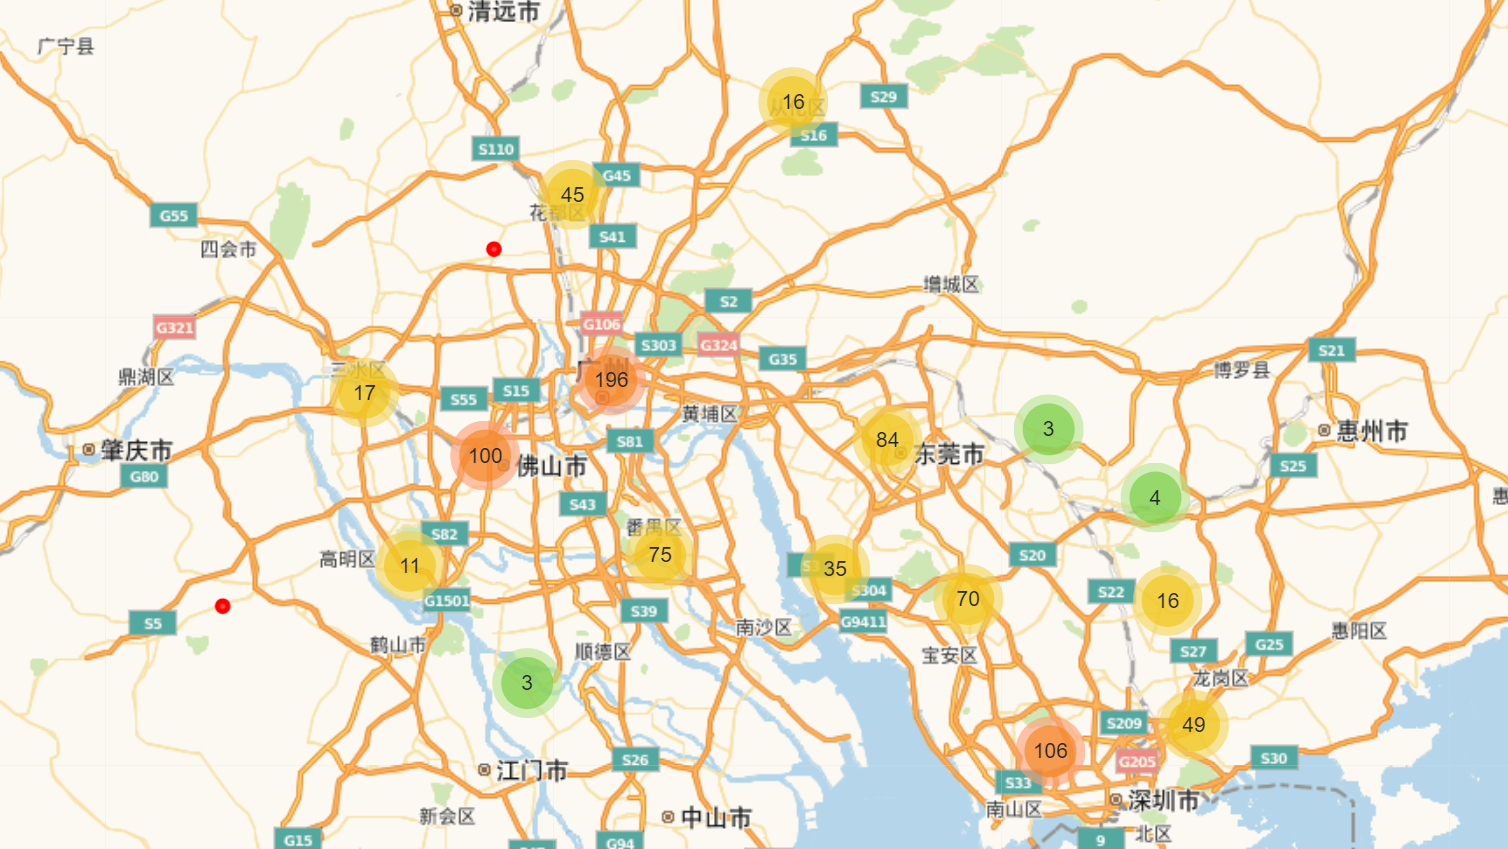
\includegraphics[width=0.7\textwidth]{renwu} %插入图片,[]中设置图片大小,{}中是图片文件名
        \caption{任务在地图上的位置示意图} %最终文档中希望显示的图片标题
        \label{Fig.main1} %用于文内引用的标签
        \end{figure}
        
        \subsubsection{定价影响因素}
        在探究定价影响因素时,我们基于 “拍照赚钱” 模式的实际运作逻辑,排除了任务发布时间、有效期等暂不可量化因素,重点聚焦于可观测的空间与用户特征。
        假设任务的复杂程度均相同,明确影响定价的关键因素可分为任务分布特征、会员分布特征两大类别,
        而会员的分布特征又包括会员信誉、会员位置两方面。
        \subsubsection{建立定价规律}
        认为任务定价$ P_i $由三部分组成:
        \begin{equation}
        Pr_i=P_0\cdot\frac{1}{1+\sum ax_i}\cdot\frac{1}{1+\sum by_iz_i}
        \end{equation}
        $ P_0 $为底价,定义任务密集程度 $TD_i= \sum x_i $、会员密集程度 $MD_i= \sum y_i z_i $作为动态调整因子。其中,$x_i$、 $z_i$可由高斯径向基函数求出,$y_i$为会员对应预定限额数。
         \begin{equation}
        x_i=e^{\frac{-d_i^2}{2\sigma_{1}^{2}}} 
        \end{equation}
        \begin{equation}
        z_i=e^{\frac{-d_i^2}{2\sigma_{2}^{2}}}
        \end{equation}
        $d_i$分别为任务与任务间、任务与会员间的距离;$\sigma _1$、$\sigma _2=0.25$。高斯核函数作为空间衰减权重,对距离赋权重。\par
        该模型基于经济学中的边际效用递减原理和空间众包任务分配中的密度惩罚机制,具有明显空间上的非线性调节结构。\par
        边际效用递减原理指随着某种经济要素消费量的增加,其带来的额外效用会逐渐减弱。
        在本模型中,这一原理主要通过任务周边会员密度(\(MD_i\))和任务密度(\(TD_i\))对定价的影响机制体现:
        对于会员密度(\(MD_i = \sum y_i z_i\)),当任务周边会员数量较少时,每新增一名会员对任务被接取的促进作用显著,此时定价可适当降低;
        但随着会员密度增大,新增会员带来的边际效用逐渐衰减 —— 即会员间的竞争加剧,即使再增加会员,对任务完成率的提升也有限,因此定价受其影响的幅度会逐步缩小。
        对于任务密度(\(TD_i = \sum x_i\)),当某一区域任务数量较少时,新增任务会显著提升区域内任务的稀缺性,定价需适当提高以吸引会员;但当任务密集到一定程度后,任务间的竞争加剧,新增任务对定价的抬升作用会减弱,符合 “边际效用随数量增加而递减” 的规律。模型公式中,\(\frac{1}{1+a \cdot MD_i}\)和\(\frac{1}{1+b \cdot TD_i}\)的分式结构直观反映了这一特性:当\(MD_i\)或\(TD_i\)增大时,分母的增长速率逐渐放缓,使得其对定价的调节力度呈现边际递减趋势,与边际效用递减原理高度契合。\par
        将附件一中的数据带入,用最小二乘法进行拟合训练可得到 $ P_0 $、 $ a $、 $ b $。\par

        \begin{table}[htbp]
        \centering
        \caption{拟合参数表}
        \begin{tabular}{lcc}
            \toprule
            \textbf{参数} & \textbf{值} & \textbf{不确定度} \\
            \midrule
            $a$ & $0.0002$ & $0.0000$ \\
            $b$ & $0.0042$ & $0.0005$ \\
            $P_0$ & $73.0725$ & $0.2715$ \\
            \bottomrule
        \end{tabular}
        \label{tab:fit_params}
        \end{table}

        由于实际任务存在实地拍摄难度差异(如超市货架核查需区分单品与多品、户外场景需考虑天气影响等),任务的完成难易程度不同,
        我们引入任务难易程度\(H_i\)以修正模型,根据上述定价公式算出的价格与实际定价的差值即为$ H_i $。
        故定价规律为:
        \begin{equation}
        Pr_i=P_0\cdot\frac{1}{1+a\cdot MD_i}\cdot\frac{1}{1+b\cdot TD_i}+H_i
        \end{equation}
        \subsubsection{分析任务未完成的原因}
        在上述定价规律分析的过程中,我们并未考虑地区差异带来的影响。
        将附件一任务完成情况进行\textit{ K-means }聚类分析,并将坐标标注在地图中。
        \begin{figure}[H] %H为当前位置,!htb为忽略美学标准,htbp为浮动图形
        \centering %图片居中
        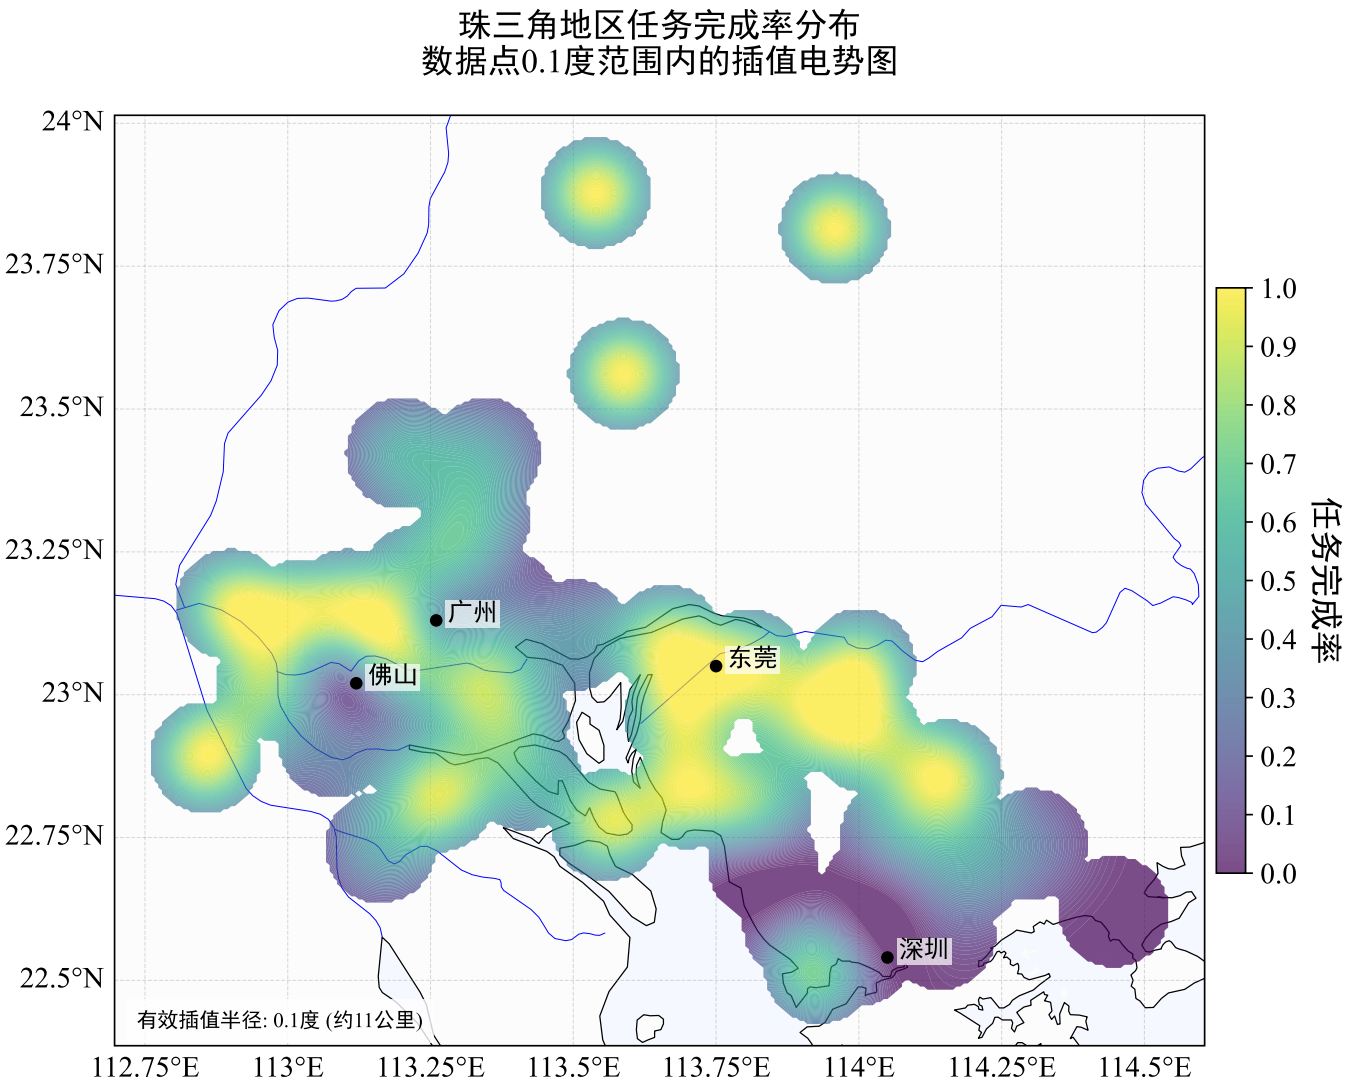
\includegraphics[width=0.7\textwidth]{kmeans} %插入图片,[]中设置图片大小,{}中是图片文件名
        \caption{任务在地图上的位置示意图} %最终文档中希望显示的图片标题
        \label{Fig.main2} %用于文内引用的标签
        \end{figure}
        由图,我们可以发现:未完成的任务主要集中在深圳市,而东莞市的任务则大多都被完成了。
        进一步结合两地经济数据可知,这样的现象与地区经济情况有关,深圳市的经济发展明显强于东莞市,居民收入水平较高,这使得深圳市的会员对任务酬金的期望阈值显著高于东莞,当任务定价低于当地会员的心理预期时,其接取意愿大幅下降,最终导致大量任务因缺乏吸引力而未被完成。
        \par 分别计算不同价格区间任务完成率并绘制图象,总的来说,可以认为在任务价格较低时,完成率也较低,而在价格逐渐增大时,完成率也随之增加。会员在选择任务时存在明显的 “趋利性”—— 在同等条件下,更倾向于接取定价较高的任务,所以部分定价较低的任务未被完成。
        \begin{figure}[H] %H为当前位置,!htb为忽略美学标准,htbp为浮动图形
        \centering %图片居中
        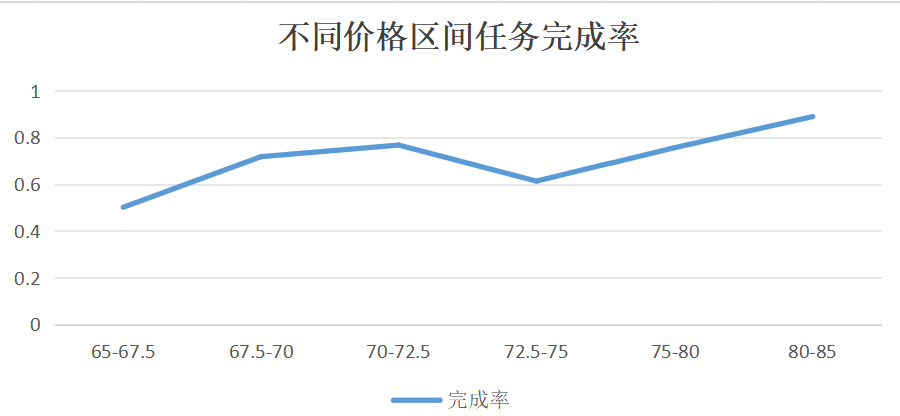
\includegraphics[width=0.7\textwidth]{wanchenglv} %插入图片,[]中设置图片大小,{}中是图片文件名
        \caption{不同价格区间任务完成率折线图} %最终文档中希望显示的图片标题
        \label{Fig.main3} %用于文内引用的标签
        \end{figure}
        \par 由此,可以得出任务未完成的几个主要原因:
        \begin{enumerate}[
        label = (\arabic*),
        itemindent = 0pt,
        labelindent = \parindent,
        labelwidth = 2em,
        labelsep = 5pt,
        leftmargin = *]
        \item 定价时未考虑地区差异,经济发展程度高地区的会员对于收益的期望较高,现
        有的定价不足以吸引他们来完成任务。
        \item 任务本身定价较低,无法达到会员期望,会员总是倾向于去完成高收益的任务。
        \item 若某任务实际难度远超定价所匹配的水平(即\(H_i\)异常偏高),即使定价合理,会员可能因完成成本(时间、精力)过高而放弃接取,导致任务未完成。
        \item 任务周围会员密度过低,若任务周边会员数量少(即\(MD_i\)过小),即使定价符合地区差异和绝对水平,也可能因 “附近无足够会员关注” 而无人接取,最终导致任务未完成。
        \item  任务周围任务密度过高导致竞争过度,若某区域大量任务集中(即任务密度\(TD_i\)过大),会员选择空间大,可能优先接取更优(如性价比更高、距离更近)的任务,导致部分任务因 “竞争劣势” 被忽略,最终未完成。
        \end{enumerate}
        \subsection{问题二}
        \subsubsection{模型建立}
        通过问题一中的分析,我们发现使得任务未完成的一个重要原因是在定价时未充分考量地区经济发展水平的差异,导致高收入地区任务吸引力不足,这是目前定价方案所存在的最大不足。
        基于上述原因,我们根据任务所处位置按城市划分为四个地区,引入地区系数$E_i$这一概念,该系数用以衡量一个地区经济发展水平
        \begin{equation}
        E_i=\frac{Q_i}{Q}
        \end{equation}
        其中,$Q_i$为地区平均收入,$Q$为总平均收入。\par
        建立新的定价模型如下:
        \begin{equation}
        Pr_{i}^{'} = \left (P_0\cdot\frac{1}{1+a\cdot PD_i}\cdot\frac{1}{1+b\cdot TD_i}+H_i\right ) \cdot E_i 
        \end{equation}
        在该模型中,假设任务价格总和不变,以任务完成率之和最高为目标。
        核心逻辑是:经济发展水平高的地区(如深圳),任务定价按系数上浮,以匹配当地会员的收入预期;而经济水平较低的地区(如东莞),定价适当下调,在控制成本的同时保证任务吸引力。模型同时遵循 “任务价格总和不变” 的约束(即 \(\sum Pr_i' = \sum Pr_i\)),确保优化方案的经济性与可行性。\par
        为衡量新定价方案的效果,我们通过 “会员满意度 - 接取率 - 完成率” 的传导链条量化任务完成情况。
        会员是否接取一个任务,与其对于任务的满意度有关,而满意度主要取决于任务的定价、
        会员与该任务的距离、任务的难易程度,以及会员所处地区的平均收入。
        综合考量以上因素,我们定义会员j对任务i的满意度为:
        \begin{equation}
        S_{ij}=\frac{P_{i}^{'}}{\left(d_{ij}+h_i\right) \cdot E_i}
        \end{equation}
        其中,$d_{ij}$为会员$j$与任务$i$之间的距离,$h_{i}$为经过离散化处理后的任务难易程度。这一结构符合经济学中“效用=收益/成本”模型逻辑,当收益增大、成本降低时,会员满意度提高。\par
        设:
        \begin{equation}
        P_{ij}=\alpha\cdot S_{ij}+ \beta 
        \end{equation}
        \par 又有:
        \begin{equation}
        \left\{
            \begin{aligned}
            1=\alpha\cdot max\left\{S_{ij}\right\} + \beta\\
            0=\alpha\cdot min\left\{S_{ij}\right\} + \beta   
            \end{aligned}
        \right.
        \end{equation}
        即可对满意度$S_{ij}$进行归一化处理,得到任务接取率$P_{ij}$,
        假设会员在接取任务后一定会将其完成,那么任务完成率$F_i$为:
        \begin{equation}
        F_i=1-\prod_{j} \left ( 1-R_{ij} \right ) 
        \end{equation}
        以任务完成率之和最大为目标函数,即:
        \begin{equation}
        max\sum_{i=1}^{n1}\sum_{j=1}^{n2}P_{ij}
        \end{equation}
        确定约束条件:
        \begin{enumerate}[
        label = (\arabic*),
        itemindent = 0pt,
        labelindent = \parindent,
        labelwidth = 2em,
        labelsep = 5pt,
        leftmargin = *] 
        \item 所有任务价格总和为定值,即:
        \[\sum P_{i}^{'} =C\]
        \item 考虑到会员完成任务的能力有限,定义新的任务限额$y_{i}^{'}$,其最大值不超过10,即:
        \[
        \sum y_{i}^{'}=
        \begin{cases}
        10& \text{ $ y_i>10 $ } \\
        y_i&\text{ $ y_i\leqslant 10 $ }
        \end{cases}
        \]
        \item 由实际情况可知,$P_0$、$a$、$b$均为正数,即:
        \[P_0>0\] \[a>0\] \[b>0\]

        \item 
        \[TD_i= \sum x_i \left(x_i<5\right) \]
               \[MD_i= \sum y_iz_i \left(z_i<5\right) \]
        \end{enumerate}
        综上所述,建立优化模型如下:
        \[ max\sum_{i=1}^{n1}\sum_{j=1}^{n2}P_{ij}\]
       \begin{equation*}
\begin{split}
&s.t.\quad  \left\{\begin{array}{lc}
\sum P_{i}^{'} =C\\
\sum y_{i}^{'}=
        \begin{cases}
        10& \text{ $ y_i>10 $ } \\
        y_i&\text{ $ y_i\leqslant 10 $ }
        \end{cases}\\
P_0>0\\
a>0\\
b>0\\
TD_i= \sum x_i \left(x_i<5\right)\\
MD_i= \sum y_iz_i \left(z_i<5\right)\\
\end{array}\right.
\end{split}
\end{equation*}
        求解可得到新的定价方案。
        \subsubsection{模型求解}
        \subsubsection{与原方案比较}
        \subsection{问题三}
        \subsubsection{确定打包方案}
        问题三中提到实际情况下,多个任务可能因为位置比较集中,导致用户会争相选择,考虑将这些任务联合在一起打包发布。
        我们首先需要根据任务的位置信息判断那些任务分布较为集中,从而进行打包。
        故对附件一中所给任务的位置信息进行\textit{Descan-K-means}聚类分析,根据分类结果将任务打包。
        \subsubsection{修改定价模型}
        在对分布集中的任务进行打包处理后,打包任务集合$i$的会员满意度需反映总难度、移动成本节省及任务数量的影响。定义\(\sum h_{i}\)为包内所有任务的离散化难度之和,\(min \left\{d_{i j}\right\}\)为会员$j$与包内最近任务的距离(替代单个任务的距离,体现移动成本节省),$n$为包内任务数量,
        则会员$j$对任务集合$i$的满意度为:
        \begin{equation}
        S_{ij}^{'}=\frac{Pr_{i}^{'}}{\left( \sum h_i+min\left\{d_{ij}\right\}+n-1\right) \cdot E_i}
        \end{equation}
        以打包前后会员对任务的满意度不变为前提,可得到新的任务定价为:
         \begin{equation}
        Pr_{i}^{''}=Pr_{i}^{'}\cdot\frac{\sum h_i+min\left\{d_{ij}\right\}+n-1}{h_i+d_{ij}}
        \end{equation}
        该公式表明,若打包后综合成本(总难度 + 最近距离 + 数量修正)低于单个任务成本总和,定价可适当下调(但保证单位收益不降低);反之则需上调,以匹配用户的成本感知。
        \subsection{问题四}
        \subsubsection{模型建立}
        问题四要求给出附件三中的新项目的任务定价方案,附件三中的数据为位置信息,先将其标注在地图中。
        新项目的任务定价方案可以基于之前建立的模型:在问题二中,我们建立了以任务完成率最高为目标的定价模型;在任务三中,通过将位置较为集中的任务联合在一起打包发布,进一步优化了该模型。
        
        \subsubsection{模型求解}
        \section{模型评价}  
        \subsubsection{应用与推广}
        该模型主要适用于 “拍照赚钱” 类自助式劳务众包平台,可帮助企业优化任务定价、提高任务完成率,尤其适合需要大规模实地信息搜集的场景,如零售商品上架核查、商圈人流统计、城市设施巡检等。其在广东省广州、佛山、东莞、深圳四市的任务数据中已得到应用,验证了区域集中型众包任务的适用性。推广价值可推广至同类众包场景:如外卖配送任务分配、同城跑腿服务、网约车订单定价等,这些场景均涉及供需匹配、距离成本、密度调节”等核心问题,模型的定价逻辑和优化目标类似。
        可为企业平衡成本与用户参与度提供量化依据,尤其适合需要控制调研成本的中小企业。
        推广前需收集目标场景的实际数据,验证模型假设(如距离与实际路程的偏差),并通过试点测试优化参数。
        \subsubsection{优点}
        \begin{enumerate}[
        label = (\arabic*),
        ]
        \item 多因素综合考量,贴合实际场景\par
        模型在定价和任务完成率分析中,综合考虑了任务密度(\(TD_i\))、会员密度(\(MD_i\))、地区经济差异(\(E_i\))、任务与会员距离(\(d_{ij}\))、任务难易程度(\(H_i\)、\(h_i\))等关键因素,且通过高斯径向基函数对距离赋予衰减权重,使空间因素的影响更符合实际规律,增强了模型的科学性。
        \item 动态调节机制,兼顾成本与效率\par
        模型基于边际效用递减原理和空间众包的密度惩罚机制,通过\(TD_i\)和\(MD_i\)动态调整定价,避免了单一定价的局限性;同时,在改进方案中以 “任务完成率之和最大” 为目标,且约束 “所有任务价格总和为定值”,兼顾了企业成本控制与任务完成效率,实用性较强。
        \item 逻辑清晰,可解释性强\par
        模型通过 “定价规律→满意度(\(S_{ij}\))→接取概率(\(P_{ij}\))→完成率(\(F_i\))” 的逻辑链条,将会员行为与任务结果关联,并引入经济学 “效用 = 收益 / 成本” 模型解释会员满意度,理论基础明确、逻辑清晰。
        \end{enumerate}
        \subsubsection{缺点}
         \begin{enumerate}[
        label = (\arabic*),
        ]
        \item 假设条件存在局限性\par
        假设 “任意两点间的实际路程可以用直线距离代替”,但实际中道路阻隔、交通状况等会导致实际距离与直线距离差异较大,可能影响距离相关参数(如\(d_{ij}\)、\(x_i\)、\(z_i\))的准确性。假设 “会员在接取任务后一定会将其完成”,忽略了会员接取后因突发情况放弃任务的可能,导致任务完成率(\(F_i\))计算结果偏高。
        \item 部分因素定义与量化不足\par
        任务难易程度\(H_i\)定义为定价公式计算值与实际定价的差值,未直接关联任务的实际难度(如拍摄复杂度、核查要求等),量化方式间接且可能存在偏差。地区系数\(E_i\)仅以 “地区平均收入” 衡量经济发展水平,未考虑生活成本、行业差异等影响会员收益期望的其他因素,对地区差异的刻画不够全面。
        \end{enumerate}
        \begin{thebibliography}{9}%宽度9
            \bibitem{bib:one} ....
        \end{thebibliography}
        \begin{appendices}
            附录的内容。
        \end{appendices}
  
    %\end{document}
%\end{tcode}

根据要求,电子版论文提交时需去掉封面和编号页。可以加上 \verb|withoutpreface|  选项来实现,即:
\begin{tcode}
    \documentclass[withoutpreface]{cumcmthesis}
\end{tcode}
这样就能实现了。打印的时候有超链接的地方不需要彩色,可以加上 \verb|bwprint| 选项。

另外目录也是不需要的,将 \verb|\tableofcontents| 注释或删除,目录就不会出现了。

团队的信息填入指定的位置,并且确保信息的正确性,以免因此白忙一场。

编译记得使用 \verb|xelatex|,而不是用 \verb|pdflatex|。在命令行编译的可以按如下方式编译:
\begin{tcode}
	xelatex example
\end{tcode}
或者使用 \verb|latexmk| 来编译,更推荐这种方式。
\begin{tcode}
	latexmk -xelatex example
\end{tcode}

下面给出写作与排版上的一些建议。

\section{图片}

建模中不可避免要插入图片。图片可以分为矢量图与位图。位图推荐使用 \verb|jpg,png| 这两种格式,避免使用 \verb|bmp| 这类图片,容易出现图片插入失败这样情况的发生。矢量图一般有 \verb|pdf,eps| ,推荐使用 \verb|pdf|  格式的图片,尽量不要使用 \verb|eps| 图片,理由相同。

注意图片的命名,避免使用中文来命名图片,可以用英文与数字的组合来命名图片。避免使用\verb|1,2,3| 这样顺序的图片命名方式。图片多了,自己都不清楚那张图是什么了,命名尽量让它有意义。下面是一个插图的示例代码。
\begin{figure}[!h]
    \centering
    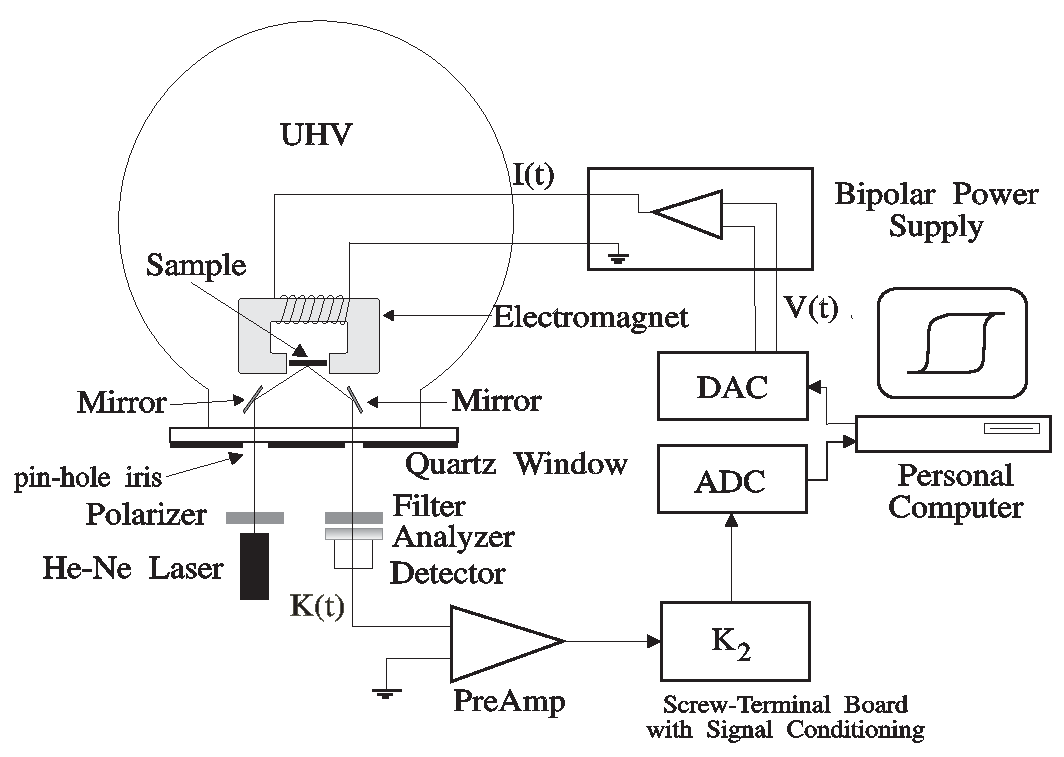
\includegraphics[width=.6\textwidth]{smokeblk}
    \caption{电路图}
    \label{fig:circuit-diagram}
\end{figure}

注意 \verb|figure| 环境是一个浮动体环境,图片的最终位置可能会跑动。\verb|[!h]| 中的 \verb|h| 是 here 的意思, \verb|!| 表示忽略一些浮动体的严格规则。另外里面还可以加上 \verb|btp| 选项,它们分别是 bottom, top, page 的意思。只要这几个参数在花括号里面,作用是不分先后顺序的。page 在这里表示浮动页。

\verb|\label{fig:circuit-diagram}| 是一个标签,供交叉引用使用的。例如引用图片 \verb|\cref{fig:circuit-diagram}| 的实际效果是\cref{fig:circuit-diagram}。图片是自动编号的,比起手动编号,它更加高效。\verb|\cref{label}| 由 \verb|cleveref| 宏包提供,比普通的 \verb|\ref{label}| 更加自动化。 \verb|label| 要确保唯一,命名方式推荐用图片的命名方式。

图片并排的需求解决方式多种多样,下面用 \verb|minipage| 环境来展示一个简单的例子。注意,以下例子用到了 \verb|subcaption| 命令,需要加载 subcaption 宏包。

\begin{figure}
    \centering
    \begin{minipage}[c]{0.3\textwidth}
        \centering
        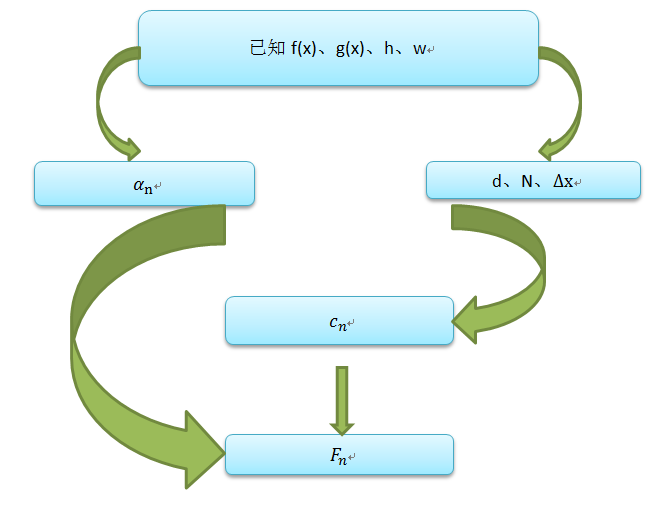
\includegraphics[width=0.95\textwidth]{f1}
        \subcaption{流程图}
        \label{fig:sample-figure-a}
    \end{minipage}
    \begin{minipage}[c]{0.3\textwidth}
        \centering
        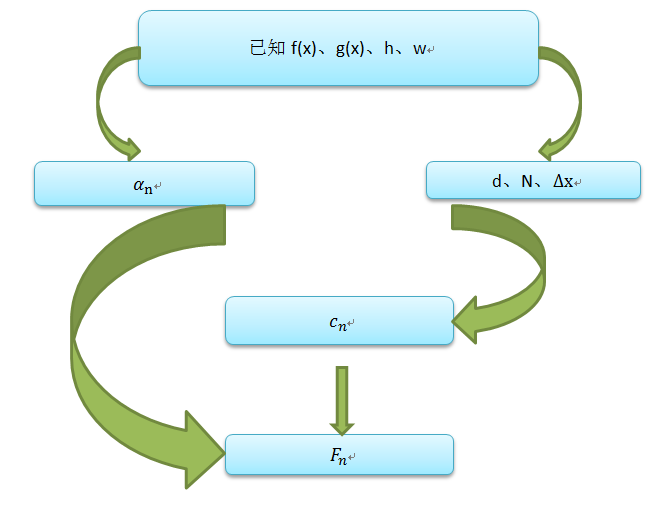
\includegraphics[width=0.95\textwidth]{f1}
        \subcaption{流程图}
        \label{fig:sample-figure-b}
    \end{minipage}
    \begin{minipage}[c]{0.3\textwidth}
        \centering
        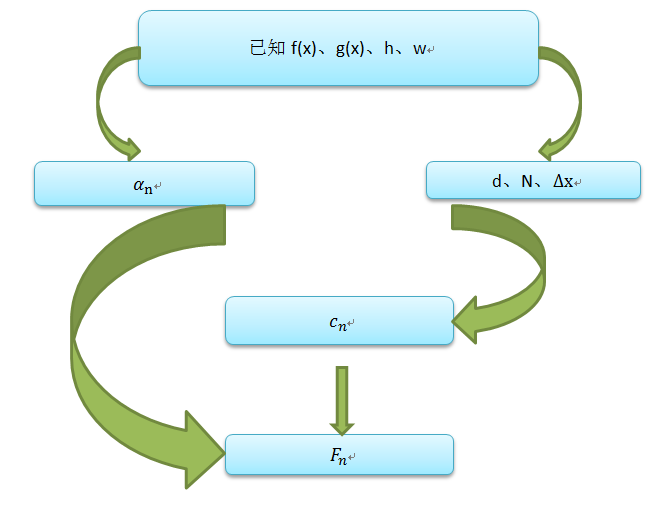
\includegraphics[width=0.95\textwidth]{f1}
        \subcaption{流程图}
        \label{fig:sample-figure-c}
    \end{minipage}
    \caption{多图并排示例}
    \label{fig:sample-figure}
\end{figure}
这相当于整体是一张大图片,大图片引用是\cref{fig:sample-figure},子图引用别分是\cref{fig:sample-figure-a}、\cref{fig:sample-figure-b}、\cref{fig:sample-figure-c}。

如果原本两张图片的高度不同,但是希望它们缩放后等高的排在同一行,参考这个例子:
\begin{figure}
    \centering
    \begin{minipage}[c]{0.48\textwidth}
        \centering
        
\includegraphics[height=0.2\textheight]{cat}
        \subcaption{一只猫}
    \end{minipage}
    \begin{minipage}[c]{0.48\textwidth}
        \centering
        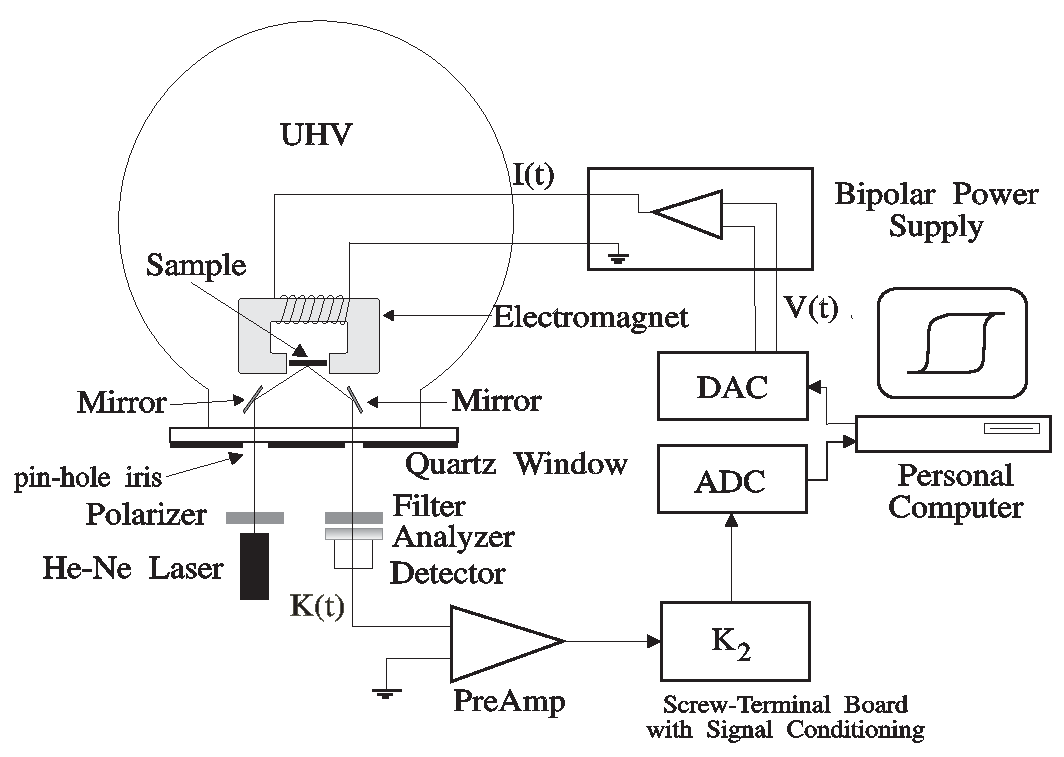
\includegraphics[height=0.2\textheight]{smokeblk}
        \subcaption{电路图}
    \end{minipage}
    \caption{多图并排示例}
\end{figure}

\section{绘制普通三线表格}
表格应具有三线表格式,因此常用 booktabs宏包,其标准格式如\cref{tab:001}~所示。
\begin{table}[!htbp]
    \caption{标准三线表格}\label{tab:001} \centering
    \begin{tabular}{ccccc}
        \toprule[1.5pt]
        $D$(in) & $P_u$(lbs) & $u_u$(in) & $\beta$ & $G_f$(psi.in)\\
        \midrule[1pt]
        5 & 269.8 & 0.000674 & 1.79 & 0.04089\\
        10 & 421.0 & 0.001035 & 3.59 & 0.04089\\
        20 & 640.2 & 0.001565 & 7.18 & 0.04089\\
        \bottomrule[1.5pt]
    \end{tabular}
\end{table}

其绘制表格的代码及其说明如下。
\begin{tcode}
    \begin{table}[!htbp]
        \caption[标签名]{中文标题}
        \begin{tabular}{cc...c}
            \toprule[1.5pt]
            表头第1个格   & 表头第2个格   & ... & 表头第n个格  \\
            \midrule[1pt]
            表中数据(1,1) & 表中数据(1,2) & ... & 表中数据(1,n)\\
            表中数据(2,1) & 表中数据(2,2) & ... & 表中数据(2,n)\\
            ...................................................\\
            表中数据(m,1) & 表中数据(m,2) & ... & 表中数据(m,n)\\
            \bottomrule[1.5pt]
        \end{tabular}
    \end{table}
\end{tcode}

\bigskip

table环境是一个将表格嵌入文本的浮动环境。tabular环境的必选参数由每列对应一个格式字符所组成:c表示居中,l表示左对齐,r表示右对齐,其总个数应与表的列数相同。此外,\verb|@{文本}|可以出现在任意两个上述的列格式之间,其中的文本将被插入每一行的同一位置。表格的各行以\verb|\\|分隔,同一行的各列则以\&分隔。 \verb|\toprule| 、\verb|\midrule| 和 \verb|\bottomrule| 三个命令是由booktabs宏包提供的,其中 \verb|\toprule| 和 \verb|\bottomrule| 分别用来绘制表格的第一条(表格最顶部)和第三条(表格最底部)水平线, \verb|\midrule| 用来绘制第二条(表头之下)水平线,且第一条和第三条水平线的线宽为 1.5pt ,第二条水平线的线宽为 1pt 。引用方法与图片的相同。

\section{公式}

数学建模必然涉及不少数学公式的使用。下面简单介绍一个可能用得上的数学环境。

首先是行内公式,例如 $ \theta $ 是角度。行内公式使用 \verb|$  $| 包裹。

行间公式不需要编号的可以使用 \verb|\[  \]| 包裹,例如
\[
E=mc^2
\]
其中 $ E $ 是能量,$ m $ 是质量,$ c $ 是光速。

如果希望某个公式带编号,并且在后文中引用可以参考下面的写法:
\begin{equation}
E=mc^2
\label{eq:energy}
\end{equation}
式\cref{eq:energy}是质能方程。

多行公式有时候希望能够在特定的位置对齐,以下是其中一种处理方法。
\begin{align}
P & = UI \\
& = I^2R
\end{align}
\verb|&| 是对齐的位置, \verb|&| 可以有多个,但是每行的个数要相同。

矩阵的输入也不难。
\[
\mathbf{X} = \left(
    \begin{array}{cccc}
    x_{11} & x_{12} & \ldots & x_{1n}\\
    x_{21} & x_{22} & \ldots & x_{2n}\\
    \vdots & \vdots & \ddots & \vdots\\
    x_{n1} & x_{n2} & \ldots & x_{nn}\\
    \end{array} \right)
\]

分段函数这些可以用 \verb|case| 环境,但是它要放在数学环境里面。
\[
f(x) =
    \begin{cases}
        0 &  x \text{为无理数} ,\\
        1 &  x \text{为有理数} .
    \end{cases}
\]
在数学环境里面,字体用的是数学字体,一般与正文字体不同。假如要公式里面有个别文字,则需要把这部分放在 \verb|text| 环境里面,即 \verb|\text{文本环境}| 。

公式中个别需要加粗的字母可以用 \verb|$\bm{math symbol}$| 。如 $ \alpha a\bm{\alpha a} $ 。

以上仅简单介绍了基础的使用,对于更复杂的需求,可以阅读相关的宏包手册,如 \href{http://texdoc.net/texmf-dist/doc/latex/amsmath/amsldoc.pdf}{amsmath}。

希腊字母这些如果不熟悉,可以去查找符号文件 \href{http://mirrors.ctan.org/info/symbols/comprehensive/symbols-a4.pdf}{symbols-a4.pdf} ,也可以去 \href{http://detexify.kirelabs.org/classify.html}{detexify} 网站手写识别。另外还有数学公式识别软件 \href{https://mathpix.com/}{mathpix} 。

下面简单介绍一下定理、证明等环境的使用。
\begin{definition}
    定义环境
    \label{def:nosense}
\end{definition}
\cref{def:nosense}除了告诉你怎么使用这个环境以外,没有什么其它的意义。

除了 definition 环境,还可以使用 theorem 、lemma、corollary、assumption、conjecture、axiom、principle、problem、example、proof、solution 这些环境,根据论文的实际需求合理使用。

\begin{theorem}
    这是一个定理。
    \label{thm:example}
\end{theorem}
由\cref{thm:example}我们知道了定理环境的使用。

\begin{lemma}
    这是一个引理。
    \label{lem:example}
\end{lemma}
由\cref{lem:example}我们知道了引理环境的使用。

\begin{corollary}
    这是一个推论。
    \label{cor:example}
\end{corollary}
由\cref{cor:example}我们知道了推论环境的使用。

\begin{assumption}
    这是一个假设。
    \label{asu:example}
\end{assumption}
由\cref{asu:example}我们知道了假设环境的使用。

\begin{conjecture}
    这是一个猜想。
    \label{con:example}
\end{conjecture}
由\cref{con:example}我们知道了猜想环境的使用。

\begin{axiom}
    这是一个公理。
    \label{axi:example}
\end{axiom}
由\cref{axi:example}我们知道了公理环境的使用。

\begin{principle}
    这是一个定律。
    \label{pri:example}
\end{principle}
由\cref{pri:example}我们知道了定律环境的使用。

\begin{problem}
    这是一个问题。
    \label{pro:example}
\end{problem}
由\cref{pro:example}我们知道了问题环境的使用。

\begin{example}
    这是一个例子。
    \label{exa:example}
\end{example}
由\cref{exa:example}我们知道了例子环境的使用。

\begin{proof}
    这是一个证明。
    \label{prf:example}
\end{proof}
由\cref{prf:example}我们知道了证明环境的使用。

\begin{solution}
    这是一个解。
    \label{sol:example}
\end{solution}
由\cref{sol:example}我们知道了解环境的使用。



\section{其它小功能}
\subsection{脚注}

利用 \verb|\footnote{具体内容}| 可以生成脚注\footnote{脚注可以补充说明一些东西}。

\subsection{无序列表与有序列表}

无序列表是这样的:
\begin{itemize}
    \item one
    \item two
    \item ...
\end{itemize}

有序列表是这样子的:
\begin{enumerate}
    \item one
    \item two
    \item ...
\end{enumerate}

\subsection{字体加粗与斜体}

如果想强调部分内容,可以使用加粗的手段来实现。加粗字体可以用 \verb|\textbf{加粗}| 来实现。例如: \textbf{这是加粗的字体。 This is bold fonts} 。

中文字体没有斜体设计,但是英文字体有。\textit{斜体 Italics}。

\section{参考文献与引用}

参考文献对于一篇正式的论文来说是必不可少的,在建模中重要的参考文献当然应该列出。\LaTeX{}在这方面的功能也是十分强大的,下面进介绍一个比较简单的参考文献制作方法。有兴趣的可以学习 \verb|bibtex| 或 \verb|biblatex| 的使用。

\LaTeX{}的入门书籍可以看《\LaTeX{}入门》\cite{liuhaiyang2013latex}。这是一个简单的引用,用 \verb|\cite{bibkey}| 来完成。要引用成功,当然要维护好 bibitem 了。下面是个简单的例子。



%参考文献
\begin{thebibliography}{9}%宽度9
    \bibitem[1]{liuhaiyang2013latex}
    刘海洋.
    \newblock \LaTeX {}入门\allowbreak[J].
    \newblock 电子工业出版社, 北京, 2013.
    \bibitem[2]{mathematical-modeling}
    全国大学生数学建模竞赛论文格式规范 (2023 年 修改).
    \bibitem{3} \url{https://www.latexstudio.net}
\end{thebibliography}

\newpage
%附录
\begin{appendices}

\section{模板所用的宏包}
\begin{table}[htbp]
    \centering
    \caption{宏包罗列}
    \begin{tabular}{ccccc}
        \toprule
        \multicolumn{5}{c}{模板中已经加载的宏包} \\
        \midrule
        amsbsy & amsfonts & {amsgen} & {amsmath} & {amsopn} \\
        amssymb & amstext & {appendix} & {array} & {atbegshi} \\
        atveryend & auxhook & {bigdelim} & {bigintcalc} & {bigstrut} \\
        bitset & bm    & {booktabs} & {calc} & {caption} \\
        caption3 & CJKfntef & {cprotect} & {ctex} & {ctexhook} \\
        ctexpatch & enumitem & {etexcmds} & {etoolbox} & {everysel} \\
        expl3 & fix-cm & {fontenc} & {fontspec} & {fontspec-xetex} \\
        geometry & gettitlestring & {graphics} & {graphicx} & {hobsub} \\
        hobsub-generic & hobsub-hyperref & {hopatch} & {hxetex} & {hycolor} \\
        hyperref & ifluatex & {ifpdf} & {ifthen} & {ifvtex} \\
        ifxetex & indentfirst & {infwarerr} & {intcalc} & {keyval} \\
        kvdefinekeys & kvoptions & {kvsetkeys} & {l3keys2e} & {letltxmacro} \\
        listings & longtable & {lstmisc} & {ltcaption} & {ltxcmds} \\
        multirow & nameref & {pdfescape} & {pdftexcmds} & {refcount} \\
        rerunfilecheck & stringenc & {suffix} & {titletoc} & {tocloft} \\
        trig  & ulem  & {uniquecounter} & {url} & {xcolor} \\
        xcolor-patch & xeCJK & {xeCJKfntef} & {xeCJK-listings} & {xparse} \\
        xtemplate & zhnumber &       &       &  \\
        \bottomrule
    \end{tabular}%
    \label{tab:addlabel}%
\end{table}%

以上宏包都已经加载过了,不要重复加载它们。

\section{排队算法--matlab 源程序}

\begin{lstlisting}[language=matlab]
kk=2;[mdd,ndd]=size(dd);
while ~isempty(V)
[tmpd,j]=min(W(i,V));tmpj=V(j);
for k=2:ndd
[tmp1,jj]=min(dd(1,k)+W(dd(2,k),V));
tmp2=V(jj);tt(k-1,:)=[tmp1,tmp2,jj];
end
tmp=[tmpd,tmpj,j;tt];[tmp3,tmp4]=min(tmp(:,1));
if tmp3==tmpd, ss(1:2,kk)=[i;tmp(tmp4,2)];
else,tmp5=find(ss(:,tmp4)~=0);tmp6=length(tmp5);
if dd(2,tmp4)==ss(tmp6,tmp4)
ss(1:tmp6+1,kk)=[ss(tmp5,tmp4);tmp(tmp4,2)];
else, ss(1:3,kk)=[i;dd(2,tmp4);tmp(tmp4,2)];
end;end
dd=[dd,[tmp3;tmp(tmp4,2)]];V(tmp(tmp4,3))=[];
[mdd,ndd]=size(dd);kk=kk+1;
end; S=ss; D=dd(1,:);
 \end{lstlisting}

 \section{规划解决程序--lingo源代码}

\begin{lstlisting}[language=c]
kk=2;
[mdd,ndd]=size(dd);
while ~isempty(V)
    [tmpd,j]=min(W(i,V));tmpj=V(j);
for k=2:ndd
    [tmp1,jj]=min(dd(1,k)+W(dd(2,k),V));
    tmp2=V(jj);tt(k-1,:)=[tmp1,tmp2,jj];
end
    tmp=[tmpd,tmpj,j;tt];[tmp3,tmp4]=min(tmp(:,1));
if tmp3==tmpd, ss(1:2,kk)=[i;tmp(tmp4,2)];
else,tmp5=find(ss(:,tmp4)~=0);tmp6=length(tmp5);
if dd(2,tmp4)==ss(tmp6,tmp4)
    ss(1:tmp6+1,kk)=[ss(tmp5,tmp4);tmp(tmp4,2)];
else, ss(1:3,kk)=[i;dd(2,tmp4);tmp(tmp4,2)];
end;
end
    dd=[dd,[tmp3;tmp(tmp4,2)]];V(tmp(tmp4,3))=[];
    [mdd,ndd]=size(dd);
    kk=kk+1;
end;
S=ss;
D=dd(1,:);
 \end{lstlisting}
\end{appendices}

\end{document} 